\chapter{Experiments: Random Geometric Graphs}
\label{ch:rgg}

% (TODO): t!
\begin{figure}[t]
  \centering
  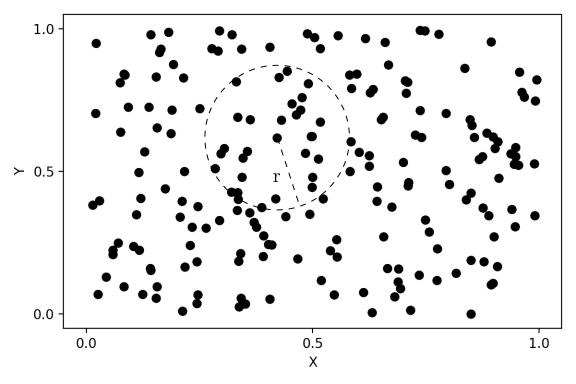
\includegraphics[width=3.5in]{figures/RGG-example.png}
  \caption{
    Example vertices drawn to generate a random geometric graph embedded in a
two-dimensional Euclidean space. The neighborhood radius $r$ of a single node is
shown.
  }
  \label{fig:rgg-example}
\end{figure}

The first idea that springs to mind when considering spatially constrained
graphs, is of course to place the vertices in some metric space. When
investigating spatial reservoirs, it is thus only natural that we begin with the
simplest spatial network model -- the random geometric graph (RGG). Figure
\ref{fig:rgg-example} depicts an example graph.

To construct a reservoir based on the RGG model, we place its $N$ internal nodes
randomly in an underlying metric space $[0, l)^{dim}$, giving each node a
position attribute sampled from a uniform distribution. For any given pair of
nodes $x, y$, we consider the Euclidean distance between them

\begin{equation}
  d(x, y) = \norm{x-y}_{2} = \sqrt{\sum_{i=1}^{dim}{(x_{i}-y_{i})^2}}.
  \label{eq:rgg-dist}
\end{equation}

Nodes are connected only to the nodes within their neighborhood radius $r$,
i.e. where $d < r$. However, since we are interested in the behavior in physical
materials, we set $r = \infty$ to allow full connectivity in all
experiments. Thus, edges are weighted according to several distance functions,
$1/d$, $1/d^2$, and $1/d^3$, to model how the interaction strength diminishes
with distance in many physical substrates. For example, the spins in artificial
spin ice is subject to a magnetic field from all neighboring spins that
diminishes according to $1/d^3$ \cite{jensen_computation_2018}. A dimensionality
of 3, i.e. $[0, l)^{3}$, is used.

\section{Size of the Underlying Volume}
\label{sec:volume-size}

\subsection{Synopsis}

Our first experiment is concerned with the size of the metric space in which we
embed the reservoir, the $l$ of $[0, l)^3$. The behavior of the ESN created will
obviously be affected by the magnitude of the weights of the network edges. A
space that is too small, will result in weights that are too big, and vice
versa.

\subsection{Results and Discussion}

% (TODO): t!
\begin{figure*}[t!]
  \centering
  \begin{subfigure}{.49\textwidth}
    \centering
    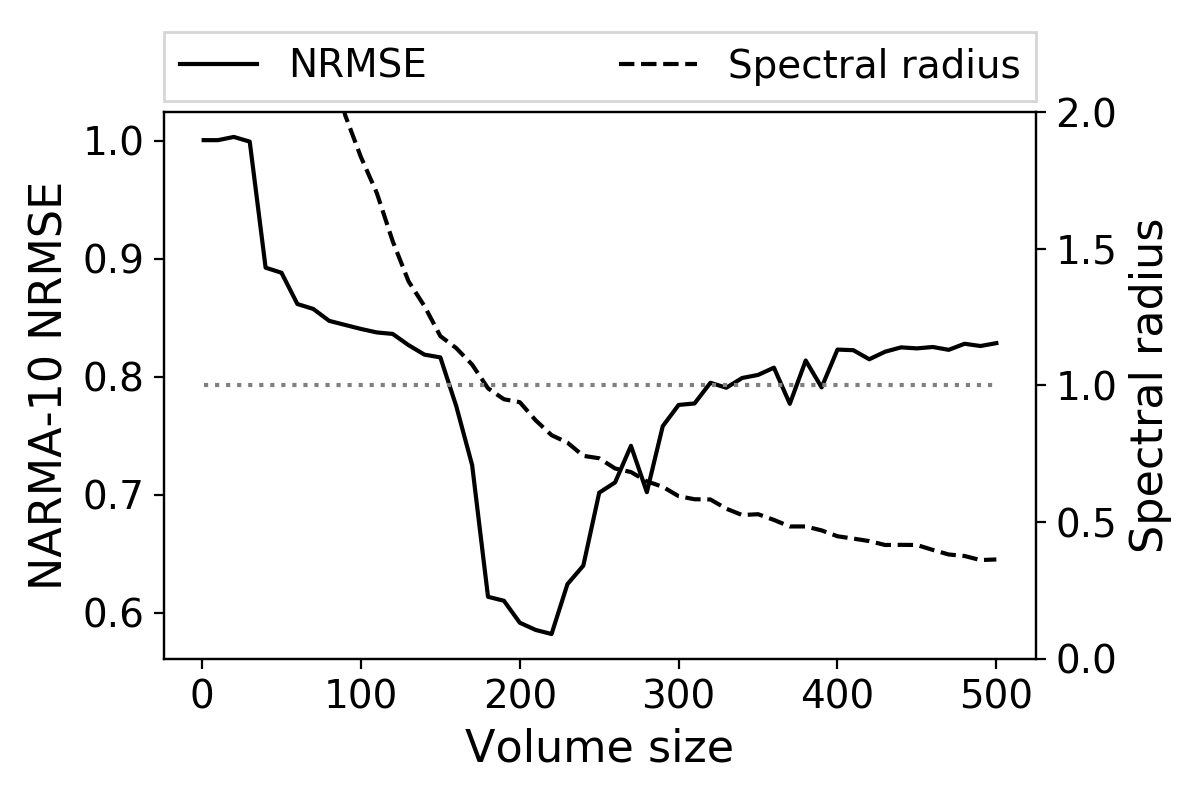
\includegraphics[width=1.0\linewidth]{figures/RGG-volume-size-inv.png}
    \caption{}
    \label{fig:size-graph-volume-a}
  \end{subfigure}
  \begin{subfigure}{.49\textwidth}
    \centering
    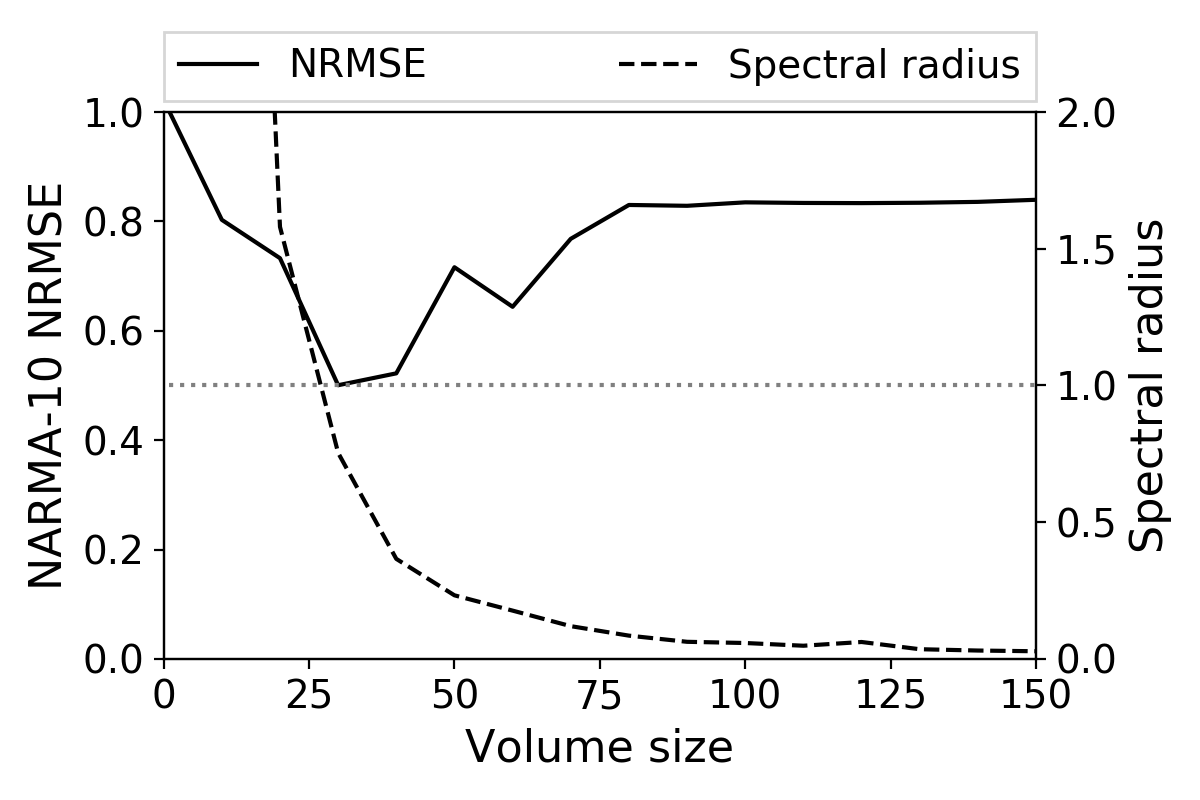
\includegraphics[width=1.0\linewidth]{figures/RGG-volume-size-inv-squared.png}
    \caption{}
    \label{fig:size-graph-volume-b}
  \end{subfigure}
  \caption{
    Spectral radius and performance of generated random geometric graphs of size
$N = 100$, as a function of the size of the underlying volume. Illustrated is
node coupling using two different distance functions: $1/d$ (a) and $1/d^2$ (b).
  }
  \label{fig:size-graph-volume}
\end{figure*}

The results of tuning the underlying volume size $l$ is shown in Figure
\ref{fig:size-graph-volume}. Shown are the results for the distance functions
$1/d$ and $1/d^2$. The plots include both the NRMSE of the network on the
NARMA-10 benchmark, and the resulting spectral radius of its internal reservoir
matrix $\mathbf{W}^{res}$ for the same network.

First, we see that an underlying volume of size $l = 1$ is near useless. The
weights generated by the $1/d$ and $1/d^2$ distance functions are too big, as
expected. The consequence of big weights is that the spectral radius of the
$\mathbf{W}^{res}$ grows too large as well. In fact, the $\tanh$ transfer
function of the internal nodes stays completely saturated throughout the entire
benchmark run.

Next, we see that as the spectral radius of $\mathbf{W}^{res}$ decreases, so
does the benchmark error. It is well-known that a spectral radius that is too
small will cause ordered or fixed-point behavior, and one that is too big may
cause unbounded deviation from initial states. Hence, the valleys seen in Figure
\ref{fig:size-graph-volume}, are equivalent to those seen in early explorations
of the spectral radius property in reservoirs
\cite{verstraeten_experimental_2007}. However, in our case, the spectral radius
is implicitly scaled by stretching the size of the underlying volume in which
the graph is embedded.

Knowledge that stretching the underlying space is equivalent to scaling them
spectral radius of the reservoir is of key interest. In physical contexts, this
means that we can scale the degree of dynamical richness in the reservoir by
moving nodes, or otherwise strengthening or lessening their connectivity. This
conclusion seems obvious, but is of importance for following experiments, as we
can directly scale the spectral radius $\mathbf{W}^{res}$ with confidence that
we could do the same by scaling the metric space.

Performance-wise, spatially constraining ESN reservoirs has caused an increase
in error compared to the non-constrained approach. The best reservoirs, seen at
the bottom of the valley in Figure \ref{fig:size-graph-volume-b}, achieve an
NRMSE around 0.5, with a spectral radius $\boldsymbol{\rho}$ around 0.8. This is
worse than what is achieved using a shift register with perfect memory. There is
thus an indication that spatial restrictions do cause a performance penalty, and
figuring out what is causing this is a main theme of the following sections.

\section{Distance Functions and Memory Capacity}
\label{sec:dist-func}

\subsection{Synopsis}

Before exploring changes to improve upon our RGG model, it is reasonable to
examine the differences between the distance functions we have available, $1/d$,
$1/d^2$, and $1/d^3$. The increasing degree of the inverse of the distance
essentially acts to reduce the neighborhood size $r$. For example, with a
distance function of $1/d^3$, nodes that are distant will have little or no
impact on each other.

Using the knowledge we gained in Section \ref{sec:volume-size}, we now also
directly scale the spectral radius of $\mathbf{W}^{res}$ to 0.9 by multiplying
it by the appropriate scalar.

\subsection{Results and Discussion}

% (TODO): t!
\begin{figure*}[t]
  \centering
  \begin{subfigure}{.49\textwidth}
    \centering
    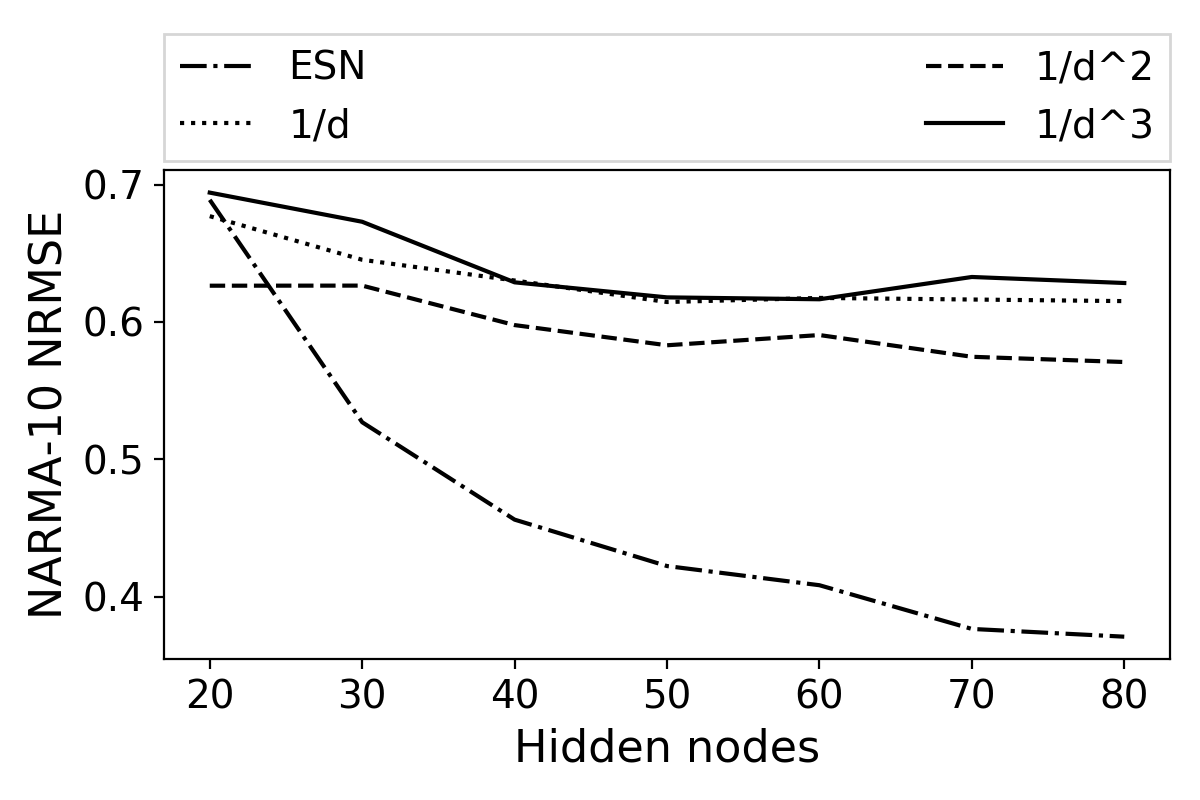
\includegraphics[width=1.0\linewidth]{figures/RGG-dist-performance-mean.png}
    \caption{}
    \label{fig:dist-performance-a}
  \end{subfigure}
  \begin{subfigure}{.49\textwidth}
    \centering
    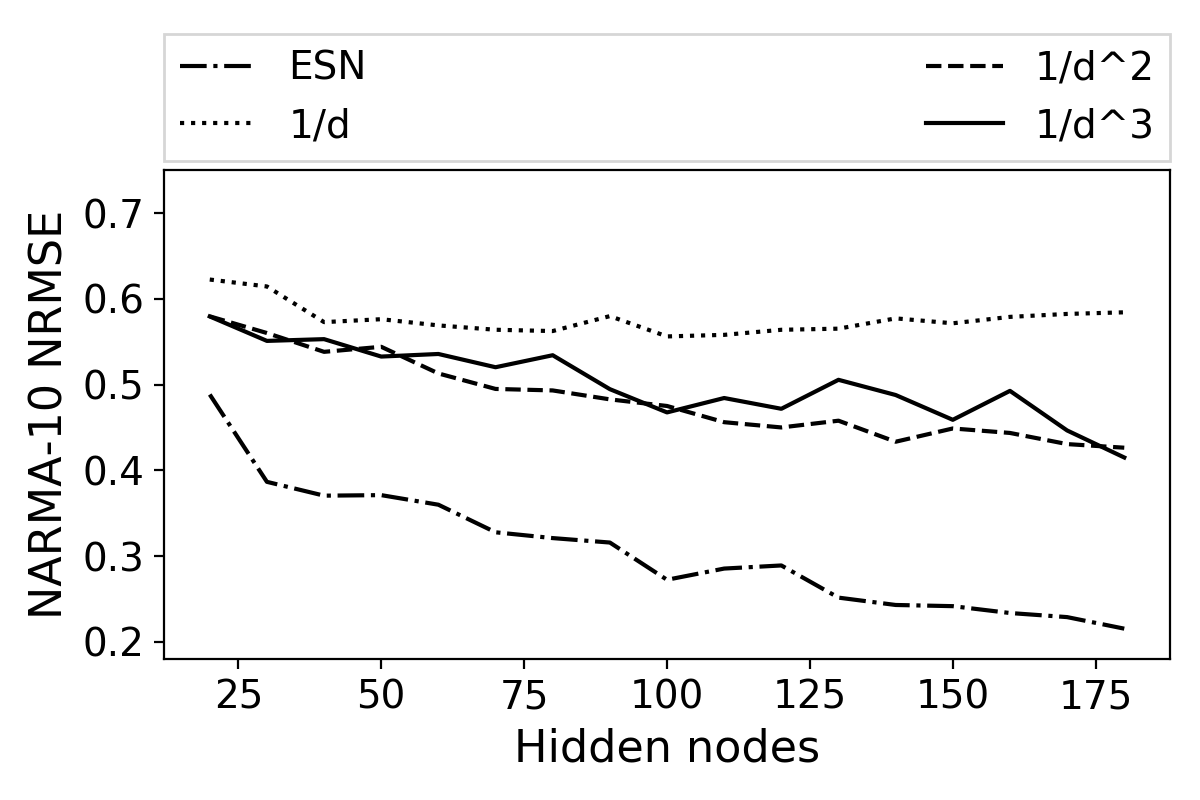
\includegraphics[width=1.0\linewidth]{figures/RGG-dist-performance-min.png}
    \caption{}
    \label{fig:dist-performance-b}
  \end{subfigure}
  \caption{
    NRMSE on the NARMA-10 task with use of different distance functions to
generate connection weights. Plots shown are the mean (a) and minimum (b) error
aggregations over 10 runs per individual parameter setup. Distance functions are
compared to the standard echo state network.
  }
  \label{fig:dist-performance}
\end{figure*}

Figure \ref{fig:dist-performance} compares the performance of the distance
functions to that of default ESNs. Plotted is NARMA-10 NRMSE as a function of
reservoir size. The average over 20 runs, shown in Figure
\ref{fig:dist-performance-a}, shows little noticeable decrease in error for the
distance functions as reservoir size increases. Additionally, it is clear that
there is some degree of variability in the error when using the $1/d^2$ and
$1/d^3$ functions. This notion is strengthened by Figure
\ref{fig:dist-performance-b}, where we see best performances for $1/d$ is about
the same as the mean, while $1/d^2$ and $1/d^3$ show a slight decrease in error
with reservoir size.

% (TODO): t!
\begin{figure*}[t]
  \centering
  \begin{subfigure}{.49\textwidth}
    \centering
    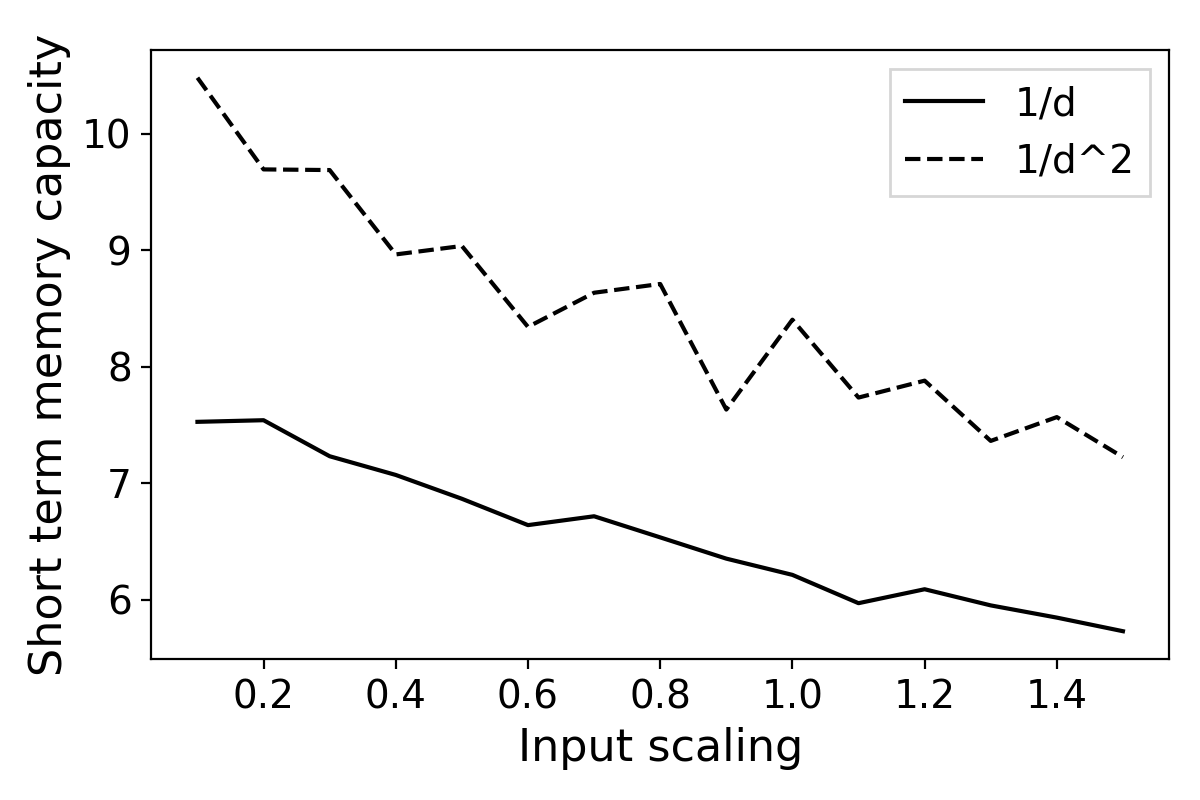
\includegraphics[width=1.0\linewidth]{figures/RGG-dist-mc.png}
    \caption{}
    \label{fig:dist-performance-is-a}
  \end{subfigure}
  \begin{subfigure}{.49\textwidth}
    \centering
    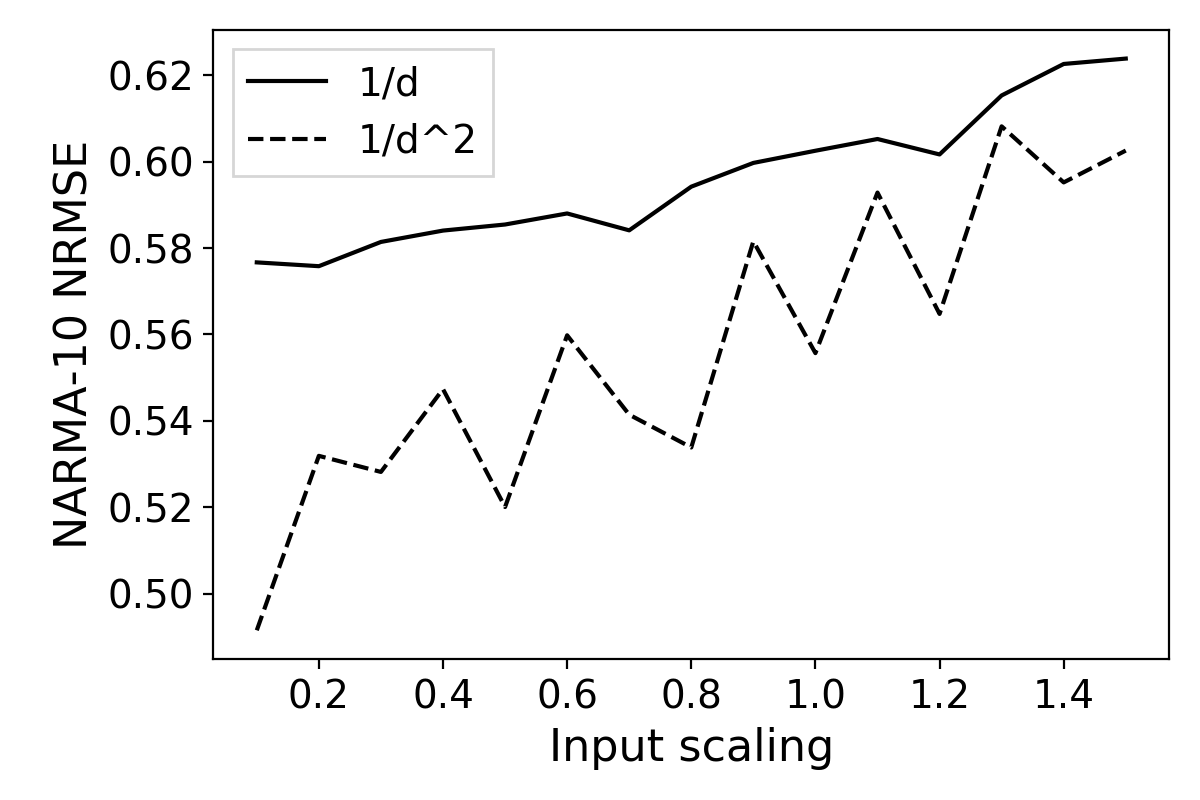
\includegraphics[width=1.0\linewidth]{figures/RGG-dist-performance-is.png}
    \caption{}
    \label{fig:dist-performance-is-b}
  \end{subfigure}
  \caption{
    Effect of input scaling on reservoirs generated as random geometric graphs,
size $N = 80$. There is a correlation between the short-term memory capacity of
the reservoirs (a), and error rates for the NARMA-10 task (b). The distance
function used is $1/d$.
  }
  \label{fig:dist-performance-is}
\end{figure*}

Empirically, we have found that reservoirs that get no significant performance
increase on the NARMA-10 task with an increasing reservoir size, tend to be
limited by memory capacity. The inability of the reservoirs to reach the
performance of a delay line supports this hypothesis. Figure
\ref{fig:dist-performance-is} highlights this, presenting both the short-term
memory capacity and the NARMA-10 NRMSE of reservoirs of size $N = 80$ as a
function of input scaling. As we decrease the input scaling, the memory capacity
increases, and error decreases. This is expected, since determines how nonlinear
the responses of the reservoir are, and there exists a memory-nonlinearity
trade-off, described in Section \ref{ssec:metrics}.

To summarize, we have found that the average performance of our distance
functions seem to hover around similar values. A general trend is that the RGG
model lacks sufficient memory capacity to solve the NARMA-10 task well,
regardless of the distance function used. Memory retention is improved by
lowering the input scaling. Further exploration can also be done by choosing a
single distance function, as our results suggest that they suffer from problems
of a similar nature.

% (TODO): I am not too happy with this section, it is a bit unclear, and might
% not be relevant/needed at all.

\section{Restoring Echo State Network Performance}

\subsection{Synopsis}

Next, we will make changes to the $\mathbf{W}^{res}$ generated with the RGG
model to move its performance close to the ESN. This may seem counter-intuitive,
as we primarily concern ourselves with physical reservoir computing. Making
arbitrary changes to the model generation is not a procedure that will
necessarily translate well to physical substrates and their restrictive
nature. However, we argue that determining the root cause of the difference in
error seen in Figure \ref{fig:dist-performance} will uncover important
properties of reservoir design. In turn, this improves our fundamental
understanding of the paradigm.

In this section, we therefore introduce signedness and directedness to the edges
of the RGG. The signedness of the reservoir is given by some fraction,
e.g. 0.10, such that each edge has a corresponding chance of becoming
negative. Reservoirs are either directed or undirected, where edges in a
directed reservoir have a 50\% chance of going in either direction. Note that
making an edge negative is not the same as reversing the direction, as it simply
means that a node will weight the value of its neighbor negatively.

For these experiments, we use the $1/d$ distance function. In Section
\ref{sec:dist-func} we found this function to give the most stable
results. Although it does not strictly produce the \textit{best} results, we
found the stability to easier to work with when looking for definitive trends in
performance. Similar results were seen with $1/d^2$, though less pronounced. We
also found lowering the input scaling to improve memory capacity, and
experiments in this section will use an input scaling of 0.1

\subsection{Results and Discussion}

% (TODO): t!
\begin{figure*}[t]
  \centering
  \begin{subfigure}{.49\textwidth}
    \centering
    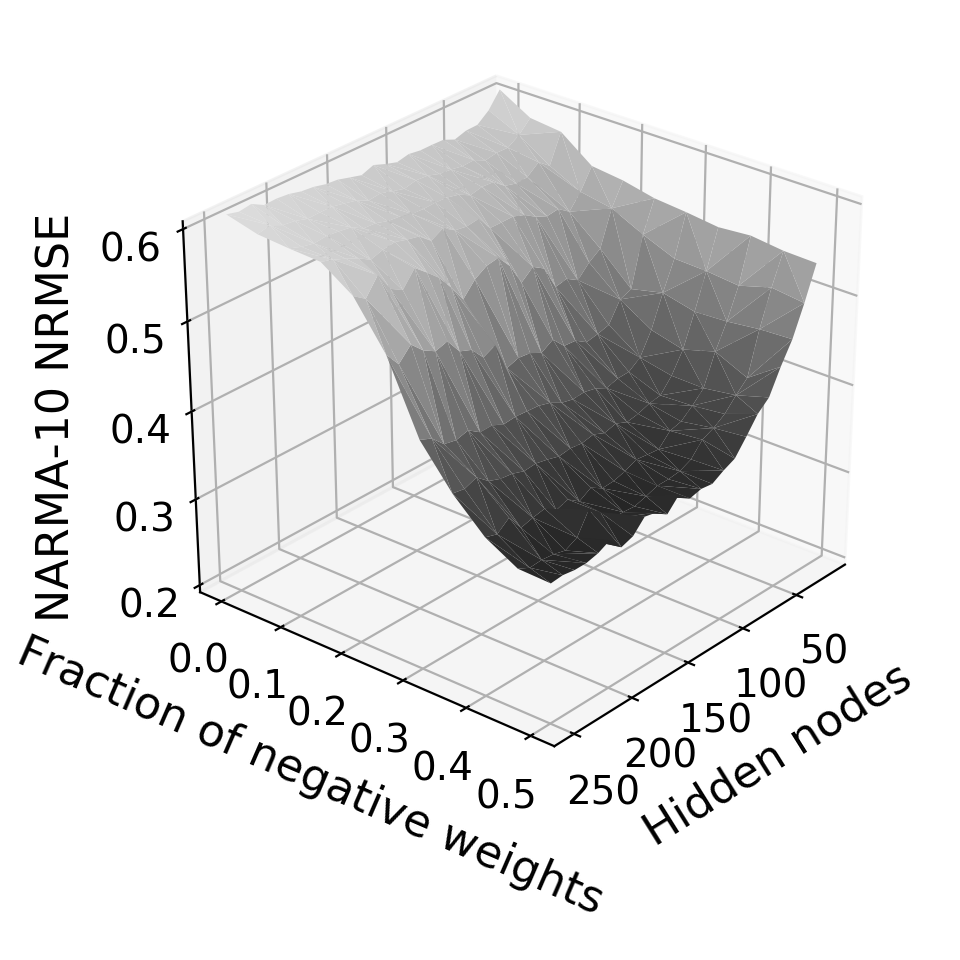
\includegraphics[width=1.0\linewidth]{figures/perf-rest-undir.png}
    \caption{}
    \label{fig:perf-restore-a}
  \end{subfigure}
  \begin{subfigure}{.49\textwidth}
    \centering
    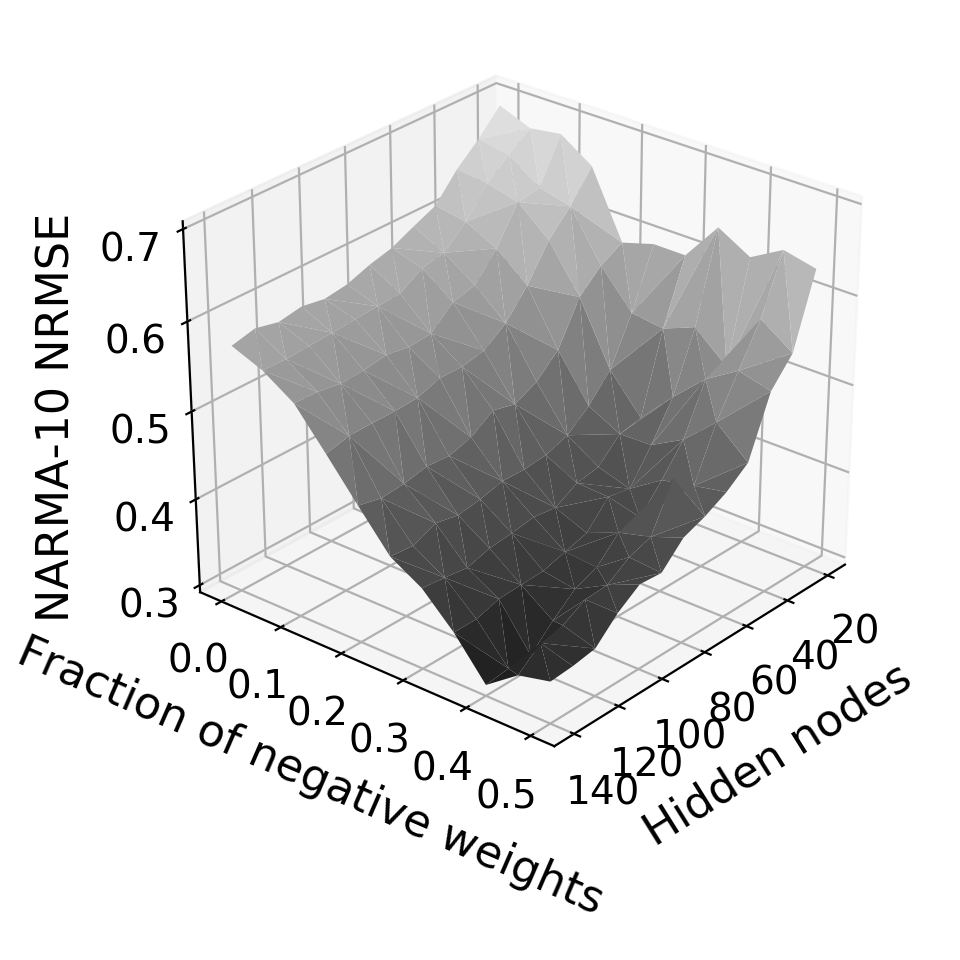
\includegraphics[width=1.0\linewidth]{figures/perf-rest-dir.png}
    \caption{}
    \label{fig:perf-restore-b}
  \end{subfigure}
  \caption{
    Introducing signed weights RGG reservoirs. Results shown are for undirected
(a) and directed (b) reservoirs.
  }
  \label{fig:perf-restore}
\end{figure*}

The impact of introducing signed, directed edges to reservoirs is shown in
Figure \ref{fig:perf-restore}. An increased fraction of signed weights decrease
the benchmark error in all cases, except for very small reservoirs. Moreover,
making the reservoir directed decreases error drastically when the fraction of
negative edges is 0.5. This is particularly true for bigger reservoirs.

Firstly, negative weights discard some of the inherent symmetry of the
network. Although the weight matrix is still symmetric in magnitude, it now
allows for a wider range of node behavior, especially considering that the lower
half of $\tanh$ becomes available. The addition of directed edges makes it clear
that a non-symmetric weight matrix enables richer dynamics, as we move below the
performance of a delay line.

% (TODO): t!
\begin{figure}[t]
  \centering
  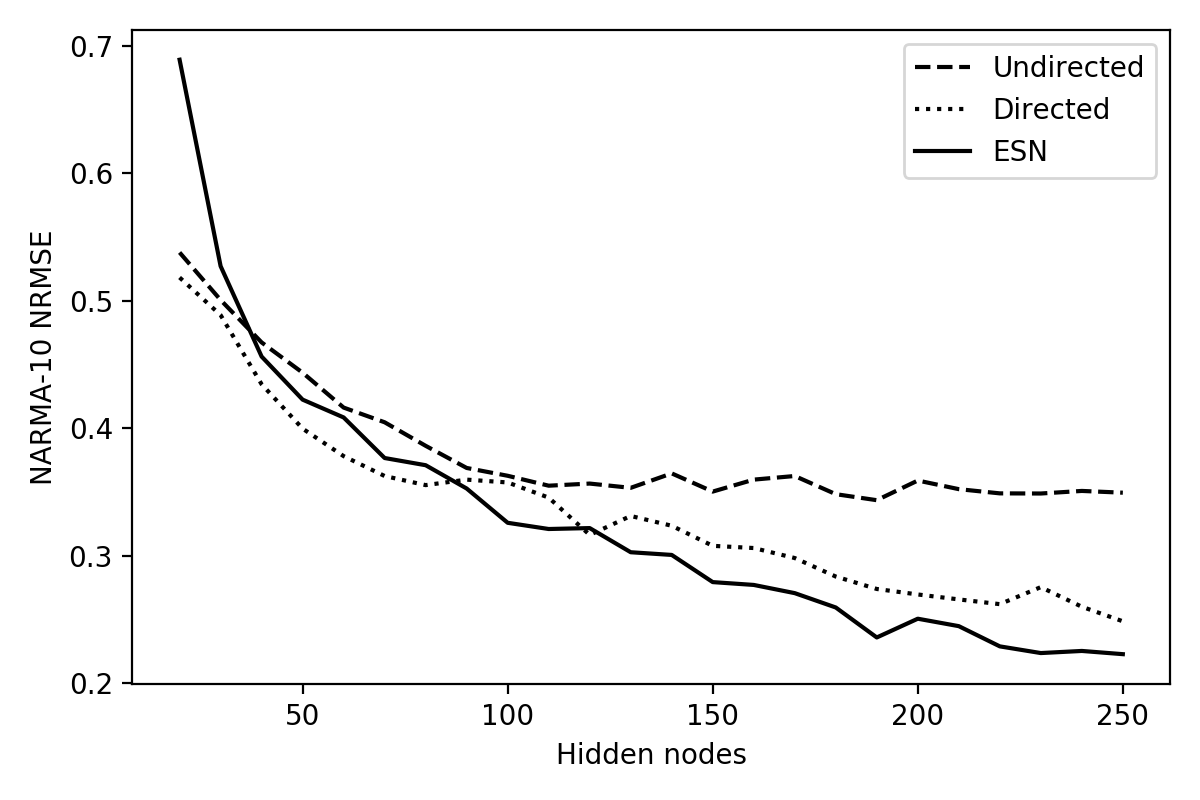
\includegraphics[width=3.5in]{figures/perf-rest-comp.png}
  \caption{
    Comparing RGG reservoirs with signed and directed edges to traditional
ESNs. Both RGG reservoirs have a fraction of negative edges of 0.5.
  }
  \label{fig:perf-rest-comp}
\end{figure}

Figure \ref{fig:perf-rest-comp} compares the performance of these reservoirs
with ESNs. Directed reservoirs with a signed weight fraction of 0.5 perform
comparably to ESNs, and scale similarly with reservoir size. Our interpretation
of this result is that the importance of \textit{flow of information} in
reservoirs should not be understated. It seems that the \textit{structure} of
the reservoir network is crucial, and that \textit{where} information flows is
more important than its magnitude.

A similar conclusion was reached in \cite{mcquillan_role_2019}, where directed
networks were shown to cover a bigger behavior space than their undirected
counterparts.

\section{Reservoir Weight Distribution}

\subsection{Synopsis}

By reintroducing signed and directed edges to the RGG model, it goes back to
resembling traditional ESNs. In fact, the major difference between the RGG model
and ESNs was their distributions of internal reservoir weights. In this section
we make a short comparison between the two.

\subsection{Results and Discussion}

% (TODO): t!
\begin{figure}[t]
  \centering
  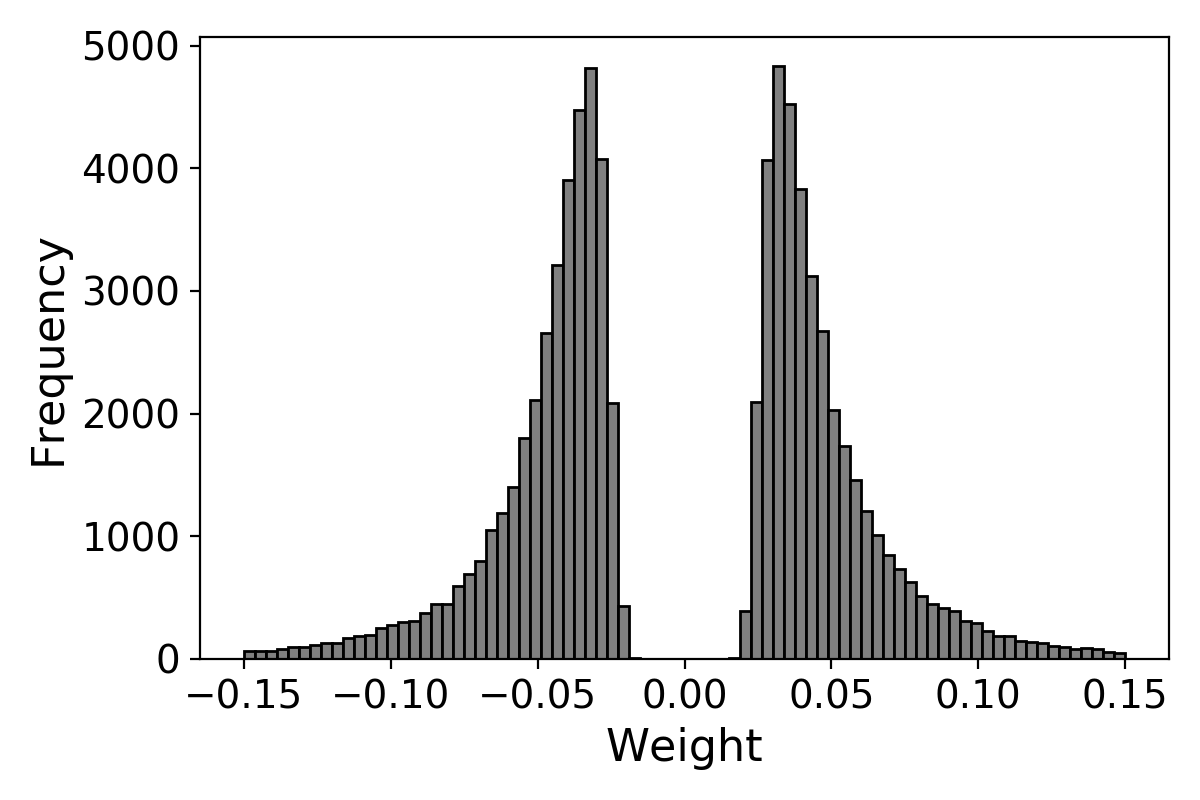
\includegraphics[width=3.5in]{figures/rgg-dist.png}
  \caption{
    Weight distribution of a reservoir with both signed and directed
edges. Zero-elements have been removed, as half of the matrix entries contain
zeroes. The distribution follows the $1/d$ distance function, which incidentally
looks similar to the reciprocal normal distribution.
  }
  \label{fig:rgg-dist}
\end{figure}

The distribution of the internal weights of RGG reservoirs with signed and
directed edges is shown in Figure \ref{fig:rgg-dist}. Three key points are worth
mentioning: (i) the distribution resembles the used distance function $1/d$,
(ii) the distribution is symmetric around zero, due to signed edges, and (iii)
elements of zero magnitude have been removed, as half of $\mathbf{W}^{res}$
contain zero-valued entries due to the directedness of the reservoir.

Distributions commonly proposed to provide ESNs with good performance include a
symmetrical uniform distribution, or a normal distribution centered around zero
\cite{montavon_practical_2012}. We end up with a symmetric distribution
resulting from the distance function $1/d$, a distribution resembling the
inverse Gaussian distribution. This distribution has, to our knowledge, not been
used in previous experiments.

Finally, we mention that the dimensionality of the underlying metric space of
the RGG plays a small role in the performance of the resulting
reservoirs. Changing the dimensionality will simply shift the weight
distribution slightly, causing little change in performance.

\section{Conclusions}

\textcolor{red}{
  The goal of.. was to..
}

\textcolor{red}{
  We have investigated imposing the simplest type of spatial restriction onto
echo state networks, and found that they by default will worsen significantly by
default. Care must be taken to ensure that the spacing between nodes will result
in node interactions that induce reservoir dynamics that are suitable for the
task at hand. This is especially important in physical reservoir computing where
the distance between nodes decides their coupling, and it can not be changed
after-the-fact.
}

% (TODO): Look more into this if found _why_ this causes this improvement,
% concretely.
\textcolor{red}{
  Further we investigated why the spatial restrictions worsened the networks
significantly, arriving at some interesting conclusions regarding flow of
information.
}

\textcolor{red}{
  Highlight the important discoveries in this chapter that lead well into the
next chapter. We would like to highlight two key discoveries: \textbf{(1)} the
fact that there are other weighting distribution schemes that work just as well
as uniform and normal, here we have discovered something that resembles the
reciprocal normal distribution using $1/d$, $1/d^2$ etc. And \textbf{(2)} that
reservoirs worsen significantly if there is no inherent flow of information,
which we in this case restored by introducing signedness and directedness to the
reservoir edges. These discoveries are important springboards into the next
chapter.
}


%%% Local Variables:
%%% mode: latex
%%% TeX-master: "../thesis"
%%% End:
